\subsection{Production}
\label{production_manual}

In our concept of Capitalism X, the production process is a grouping of various other factors. These factors are, namely: 
\begin{itemize} 
\item Products 
\item Procurement  
\item Machinery 
\item Logistics 
\item Warehousing 
\end{itemize}
You will find all of the above mentioned processes in the tabs of the production view. Each tab contains all the respective elements, that keep the production process running.
%INSERT SCREENSHOTS!!! Leave out the game mechanics part`???
The manufacturing process, which is the focus of this section is composed of several elements. Most of these elements will be visible to you through the Production view accessible in the Capitalism X game settings. Furthermore these elements, will serve as variables that will interact with each other in the game mechanics, and provide you with the appropriate indicators of performance, regarding the Production process. However other important elements will not be directly visible to you but will serve a very important role in the game mechanics. In this section we will explain all the different views and elements you can encounter whilst browsing the production view.

\subsubsection{Procurement View}
\label{sub:ProcurementView}
In order to start manufacturing or reselling goods, you need to procure the components necessary. First, you need to choose a suitable product portfolio for you. In order to do so, please go to the production area and select the procurement tab. You can see the procurement view in figure \ref{fig:procurementView}. 

\begin{figure}[h]
    \centering
    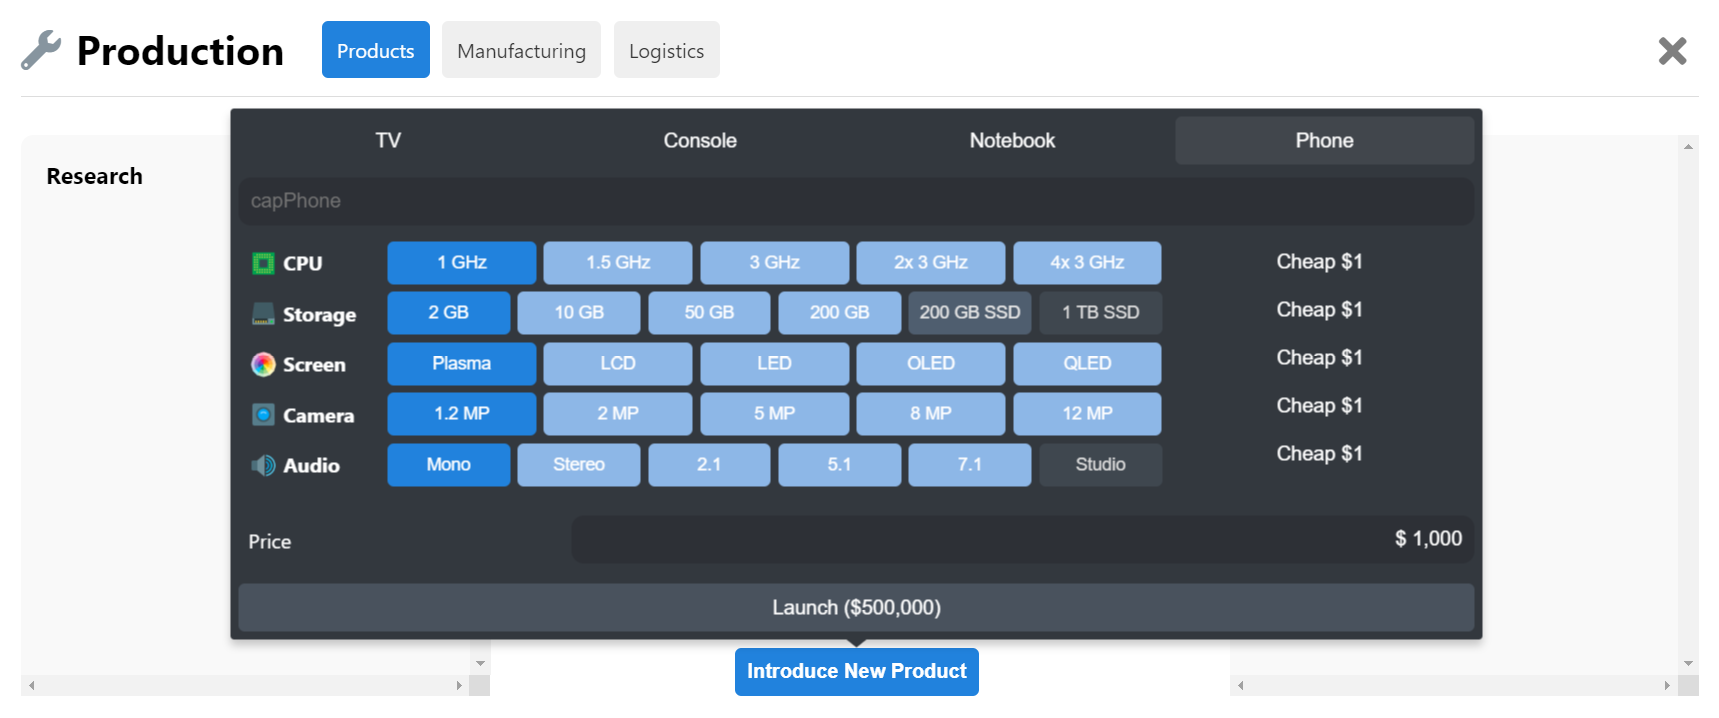
\includegraphics[width=\textwidth]{images/procurementView.png}
    \caption{Procurement view for choosing product portfolio and buying components}
    \label{fig:procurementView}
\end{figure}

There you have the possibility to add a new product to your portfolio. In the beginning, it is reasonable to start with a smaller product portfolio. In later stages of the game however, it might be interesting to test out the production and sale of different products, and maybe even different version of products, for example selling a high-quality, high-priced laptop and to compare it to selling a low-quality, low-priced laptop. Insights of such experiments might be derived from market research, sales figures, etc.

Also, you have an overview about the components the engineers need in order to manufacture a specific product. Some might be locked at the beginning and will be unlocked in due time. When clicking on a component, an overlay opens where you have the possibility to select the component from three different suppliers, which you can see in figure \ref{fig:procurementSupplier}. 
\begin{figure}[h]
    \centering
    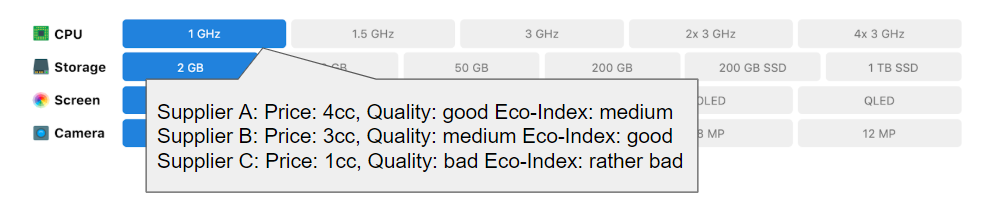
\includegraphics[width=\textwidth]{images/procurementSupplier.png}
    \caption{Choosing the supplier for a component}
    \label{fig:procurementSupplier}
\end{figure}
There are several features that help you decide which supplier to choose: the price, the eco-index and the quality index. The price varies, depending on the supplier. Next, the eco-index is a measure that defines a supplier’s ecological footprint, influenced by their logistics, sustainability in production, ecological footprint of their suppliers, and so on. This means, the components you choose might also have an influence on your company’s eco-index. Third, the quality index gives you insights about the component’s quality, so the higher the quality index, the higher the component’s quality. Again, the component’s quality has an influence on your final product’s quality index, which you should keep in mind, when defining a product’s price.

After deciding on a component from a supplier, you need to choose the amount of components you want to purchase. For a higher amount, you might get a mass discount, but beware --  buying more components than you manufacture to products may lead to higher warehousing costs. 

\subsubsection{Product View}
\label{sub:ProductView}
Now it is time to generate some revenue for your hard work! After hiring engineers, procuring the components and machinery needed, you have to decide on a market price for your respective product. In order to do so, you might go to the product view tab in the production area. There you get an overview about each product in your portfolio, which you can see in figure \ref{fig:productView}.

\begin{figure} [h]
    \centering
    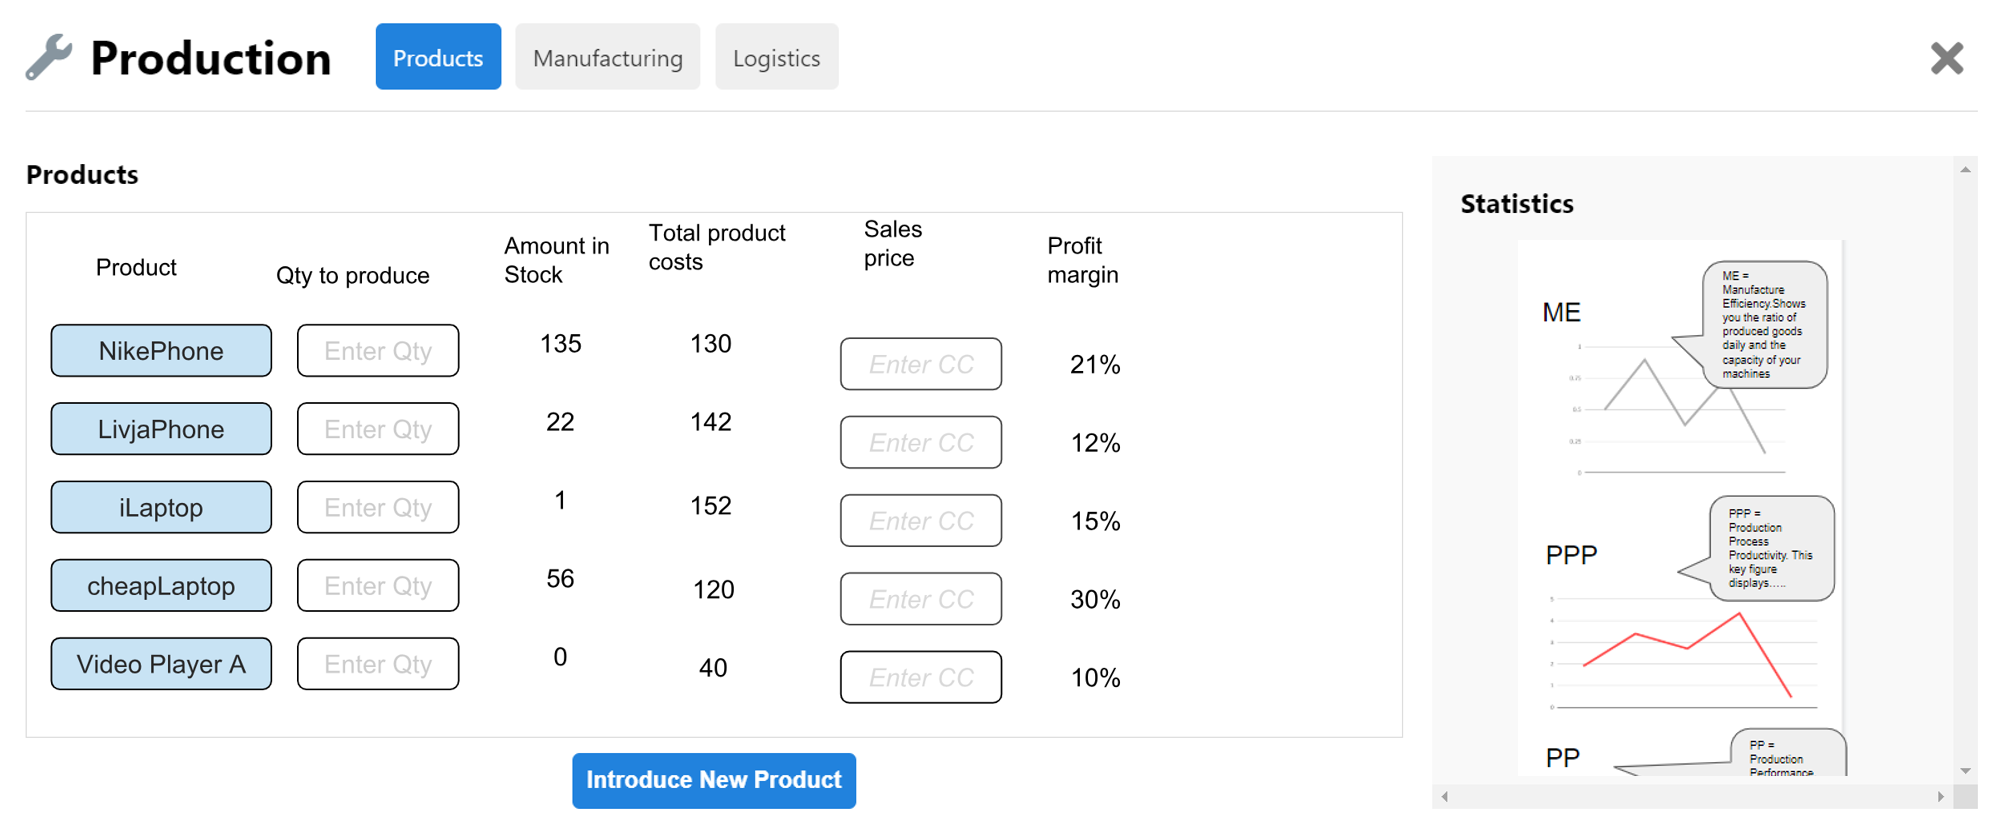
\includegraphics[width=\textwidth]{images/productView2.png}
    \caption{Product view}
    \label{fig:productView}
\end{figure}

First, you can see the product’s name, which you can adapt in the procurement view. Second, you can enter the quantity you want to produce. Next to that, you have the amount of units in stock displayed. The amount in stock will be reduced automatically when some customer buys the respective product. This means, that only if the stock is empty, products with new components will be sold to the market. However, you can produce all the time and increase the units in stock if the market is not responding yet. 

Back to the UI: next to the units in stock you can see the total product costs, which include the sum of component prices, and other fixed costs, such as electricity, and variable costs that occur during production. Based on this amount of CapCoins you might enter a market price in the next field. The respective profit margin is calculated automatically and displayed next to your defined market price. Again, market research and older sales figures may give you a hint about the reasonableness of your market price. 

With that being said, the actions you are required to take are defining the price per product in the production view. Then, as soon as you enter a quantity, the products are produced if sufficient production capacity is available. Otherwise, the products are manufactured according to the FIFO principle. After production, the products are available for purchase by your customers on the market.

\subsubsection{Machinery view} 
\label{sub:MachineryView}
Let us continue with the Machinery view, which indicates a snapshot of the current status of the company's machines. Their number and overall capacity, can be found on the right side of the tab. When looking at the center of the tab you can get a more in depth perspective of each machine. The current capacity is a value that shows the user the maximum amount of products that the machine can produce in a day. 
\begin{figure}
    \centering
    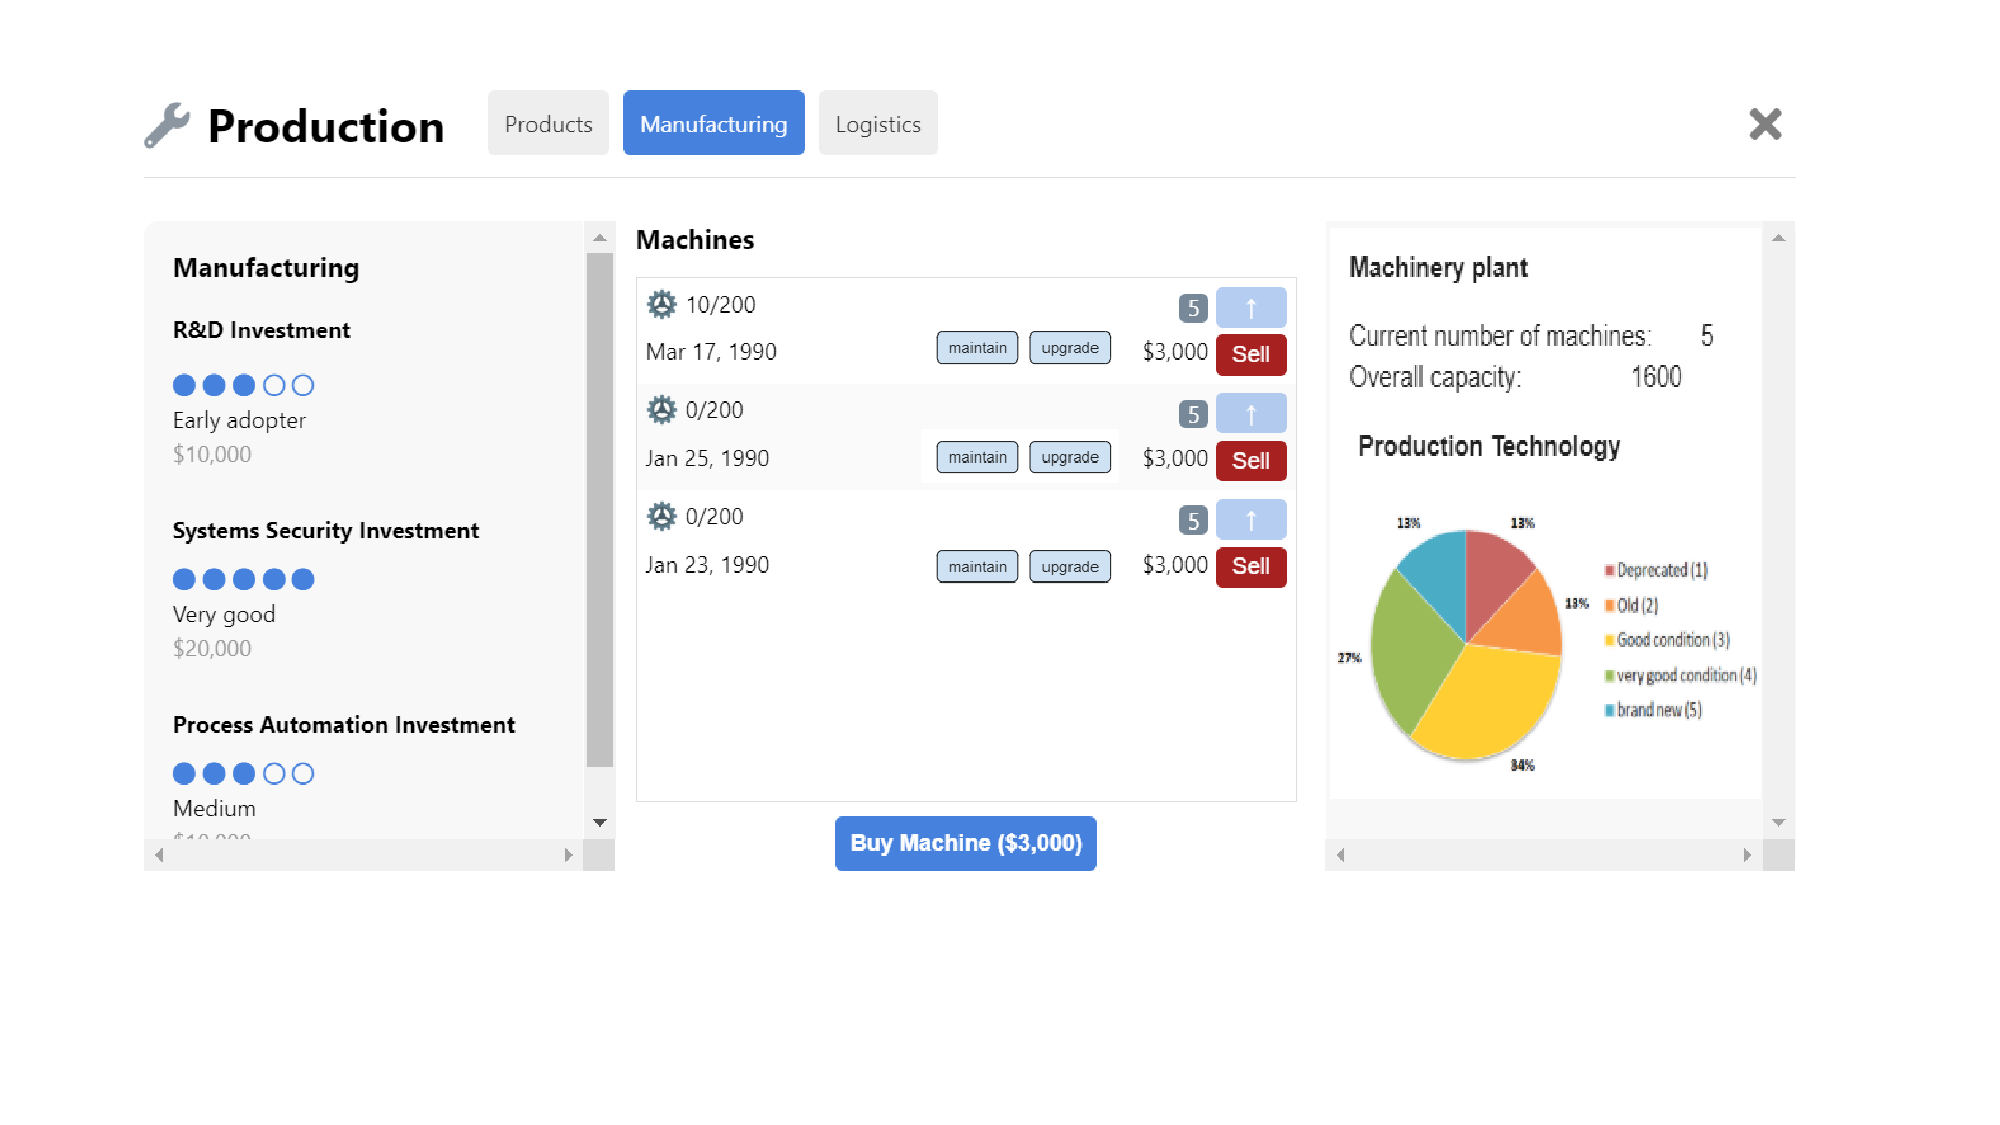
\includegraphics[width=\textwidth]{images/MachineryView.pdf}
    \caption{Prototype Machinery View}
    \label{fig:machinery view}
\end{figure}

 In the list of the individual machines, it will also be possible to maintain, upgrade and sell individual machines. The maintain and upgrade options improve the selected machinery state or in other words its production technology. 
You will also be presented with the opportunity to buy several machinery, which will all be of the same type. In the production process a machine can produce all types of products, meaning production machinery are not product specific and vice-versa. This decision has been made due to simplification of the entire production process simulation. The differences these machinery will have regard their producing capacity, and their production technology level. 

The \textit{productionTechnology} level is a value which shows the current state of a particular machinery. For this measure we developed a scale similar to the company’s general Eco-Index, but at the same time different, as it is adapted to the Production machinery.  This scale has a range from $1$ to $5$, where $1$ is a deprecated machine, and $5$ is a brand new machine. When a machine is bought it has a certain value for the technology scale, which is related closely to the price the users pay. 

The overview of this logic is represented in the actual Production view by a pie chart. We chose the pie chart as it permits a visual check of the reasonableness of the overall machine state and the differences between several states. Moreover, it is visually simpler than other types of graphs.
 
Apart from these options, there is also the possibility to sell a machine. The selling price will be determined by the game mechanics and cannot be altered by the user. This amount will be based on the capacity of the machine and its production technology level.

In the machinery view, there are also some \textit{productionInvestments} that you can make. In order to invest in R\&D, system security or process automation, you have to input the amount of CapCoins you want to invest. The amount you can input is either $0cc,5,000cc,1,0000cc,15,000cc,20,000cc$. You will have to contemplate how and what do these investment options affect, to be able to call yourself a Capitalism X pro.

\subsubsection{Performance Metrics}
This section will give you a short introduction to all the metrics that we have selected to display in the Production View. Do not be intimidated by the multiple graphs and parameters, as these metrics are your friends. They will show you everything that is happening in production, why is it happening and how well is it going. All you have to do is figure out how to keep those levels soaring. 

The first performance metric you will encounter is \textit{manufactureEfficiency} (\gls{mE}). This metric will show you how efficiently you are using your machines, in terms of units produced.
Just below manufacture efficiency you will see \textit{productionProcessProductivity}. This measure is similar to \textit{manufactureEfficiency}, because it measures efficiency, but in the same time different as it encompasses the efficiency of the entire production process. 

You will want to keep an eye on \textit{productQuality}, as this value is one of the most important in our simulation. It is influenced by a variety of factors from different departments, and in order to increase your \textit{productQuality} you have to discover and  boost them all.

Every visible metric will be generated by the game and you can not influence them directly. Step by step you will come to an understanding of how different elements in the game affect these metrics directly or indirectly.

\subsubsection{Logistic and Warehousing}
%Janine
Now that your products have been produced, it's time to take care of their delivery, as the products sold must somehow reach your customers. You can control the delivery and storage of your products in the logistics view. 
All products you produce are temporarily stored in your warehouses before they are delivered. You can either build warehouses by yourself or rent them, just as you like. If you decide to build a warehouse you can sell it later at its current value, rental contracts can be cancelled at any time. Per camp you have of course certain maintenance costs like for example electricity and also the storage of products which were not sold directly on the day of their production cause costs.

You can either arrange the delivery of your products via your own logistics fleet, outsource it to an external logistics company or combine these two options. You can easily buy trucks for your own fleet, but each truck has certain characteristics that affect the overall logistics of your company. Like the warehouses, your trucks have monthly maintenance costs. In addition, there are certain delivery costs per product. If you notice that your logistics fleet is too large and you don't need some trucks at all, you can simply sell them again at their remaining value.

Just like the trucks, in the logistics view you can also view the external logistics partners, hire them and, if desired, discharge them again. Every partner company has certain characteristics, which also affect your logistics. If you decide to work with a partner, you sign a contract, which regulates the monthly costs for the general provision of the service and the costs incurred for each package delivered. 
The figure \ref{fig:logistic_view} shows the most recent logistic and warehousing view  of the Capitalism X prototype.

\begin{figure}
    \centering
    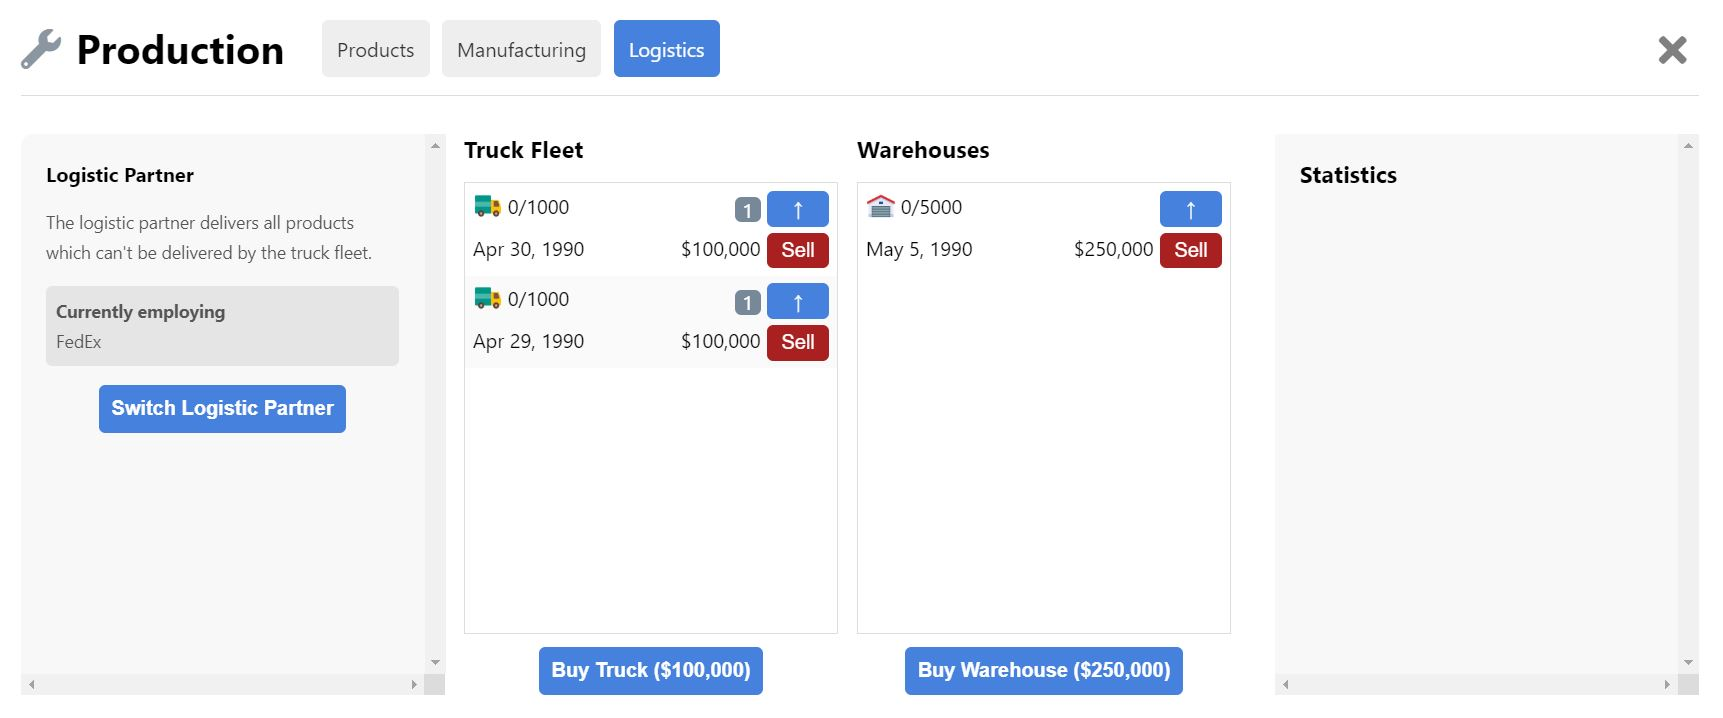
\includegraphics [width=\textwidth]{images/logistic_view.png}
    \caption{Logistic View}
    \label{fig:logistic_view}
\end{figure}